\chapter{GEOREFERENSI DATA RASTER}

Jika kita mempunyai sebuah data raster yang berasal dari hasil \textit{scanning} peta, foto udara, dan citra satelit yang belum berisi informasi yang menunjukkan referensi spasial. Kemudian kita ingin melakukan digitasi berdasarkan data \textit{raster} tersebut. Maka yang diperlukan adalah membuat peta hasil \textit{scan} tersebut mempunyai sistem koordinat dengan melakukan koreksi geometrik yaitu proses \textit{georeference}. \textit{Georeference} merupakan proses transformasi koordinat pada data \textit{raster} dari koordinat \textit{scanner} ke koordinat \textit{real-world}.

Selain foto udara dan citra satelit, data \textit{raster} bisa diperoleh melalui hasil \textit{scanning} peta analog. Peta yang baik pasti memiliki informasi koordinat geografis yang ditunjukkan dengan \textit{Grid} pada peta tersebut.

Pada Bab ini, akan dipelajari bagaimana melakukan georeferensi terhadap data \textit{raster} hasil \textit{scanning} peta analog. Untuk memulai proses georeferensi tahapan-tahapan yang dilakukan adalah sebagai berikut :

\begin{enumerate}[1.]

  \item Pada jendela utama Quantum GIS, klik \verb|Raster > Georeferencer > Georeferencer|, bila menu tersebut tidak muncul seperti gambar \ref{fig:georefmenunotexists}.
  
  \begin{figure}[H]
    \centering
    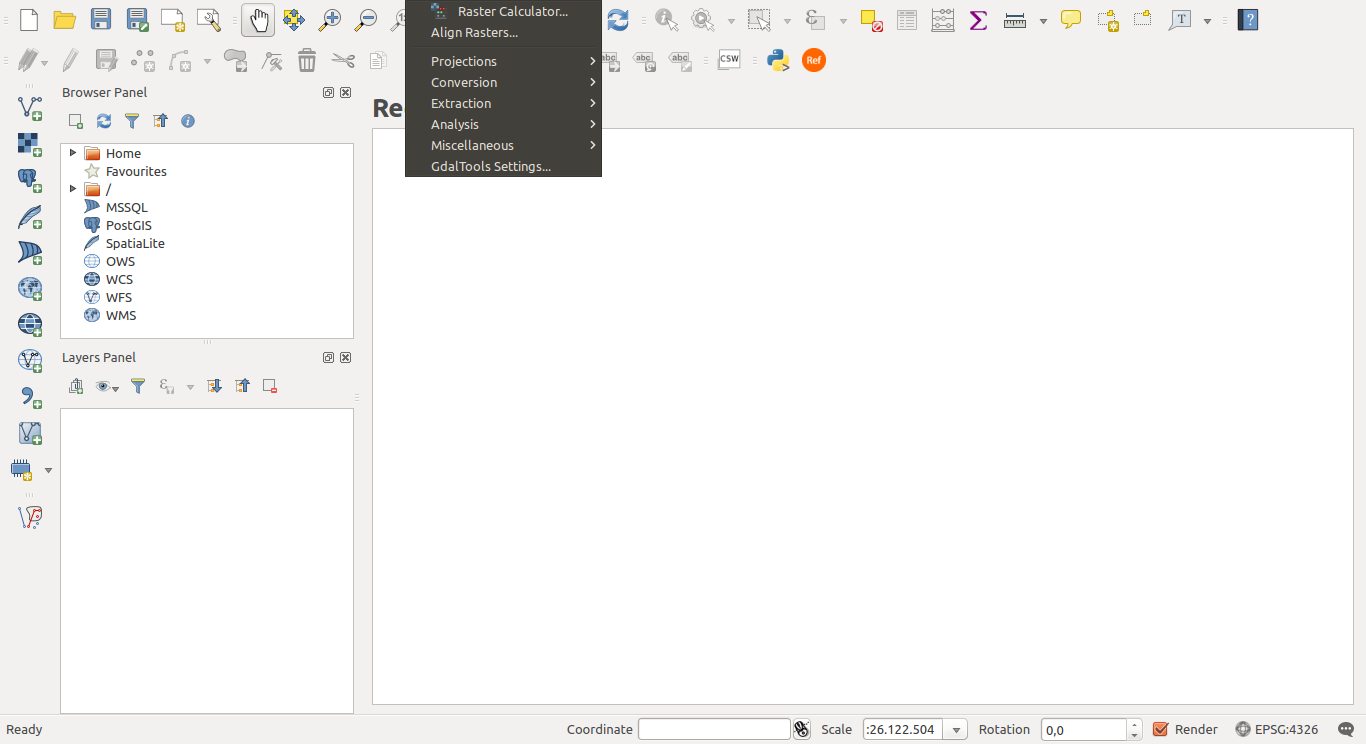
\includegraphics[width=1\textwidth]{./resources/018-menu-georeference-not-exists}
    \caption{Menu \textit{Georeference} tidak muncul}
    \label{fig:georefmenunotexists}
  \end{figure}
  
  Maka perlu memasangkan (\textit{install}) \textit{plugins} untuk \textit{georeferencer} terlebih dahulu dengan cara klik menu \verb|Plugins > Manage and Install Plugins...| sehingga muncul jendela pada gambar \ref{fig:pluginswin}.
  
  \begin{figure}[H]
    \centering
    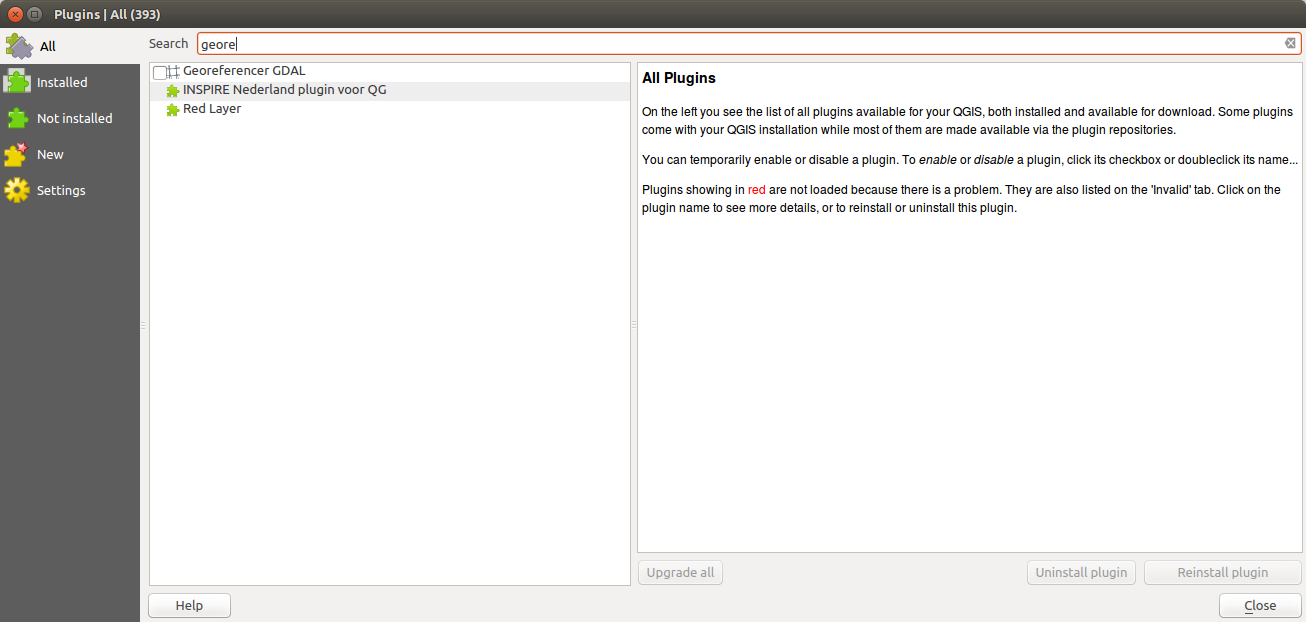
\includegraphics[width=1\textwidth]{./resources/020-pluginswin}
    \caption{Jendela \textit{Plugins}}
    \label{fig:pluginswin}
  \end{figure}
  
  sebelum jendela \textit{plugins} tersebut muncul, mungkin akan terlihat sebuah proses \textit{fetching repo} seperti pada gambar \ref{fig:fetchingrepo}.
  
  \begin{figure}[H]
    \centering
    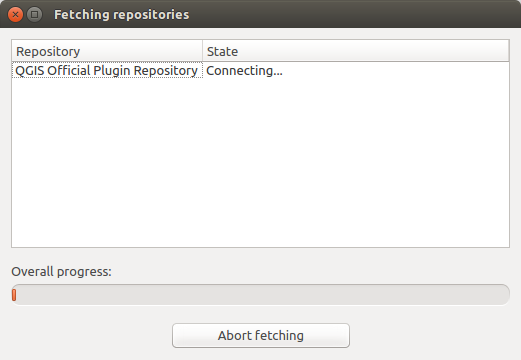
\includegraphics[width=1\textwidth]{./resources/019-fetching-repo}
    \caption{Jendela \textit{Fetching Repository}}
    \label{fig:fetchingrepo}
  \end{figure}
  
  Pada jendela \textit{plugins}, terdapat bagian \textit{search} untuk mempermudah mencari \textit{plugins} yang akan dipasang, ketikkan \verb|georeferencer| di kotak tersebut, lalu pilih tanda centang di sebelahnya. Bila belum terpasang, klik \verb|install plugin| di bagian jendela paling kanan bawah. Setelah selesai, maka akan muncul menu \verb|Georeferencer| pada menu \verb|Raster| seperti pada gambar \ref{fig:georefmenuexists}
  
  \begin{figure}[H]
    \centering
    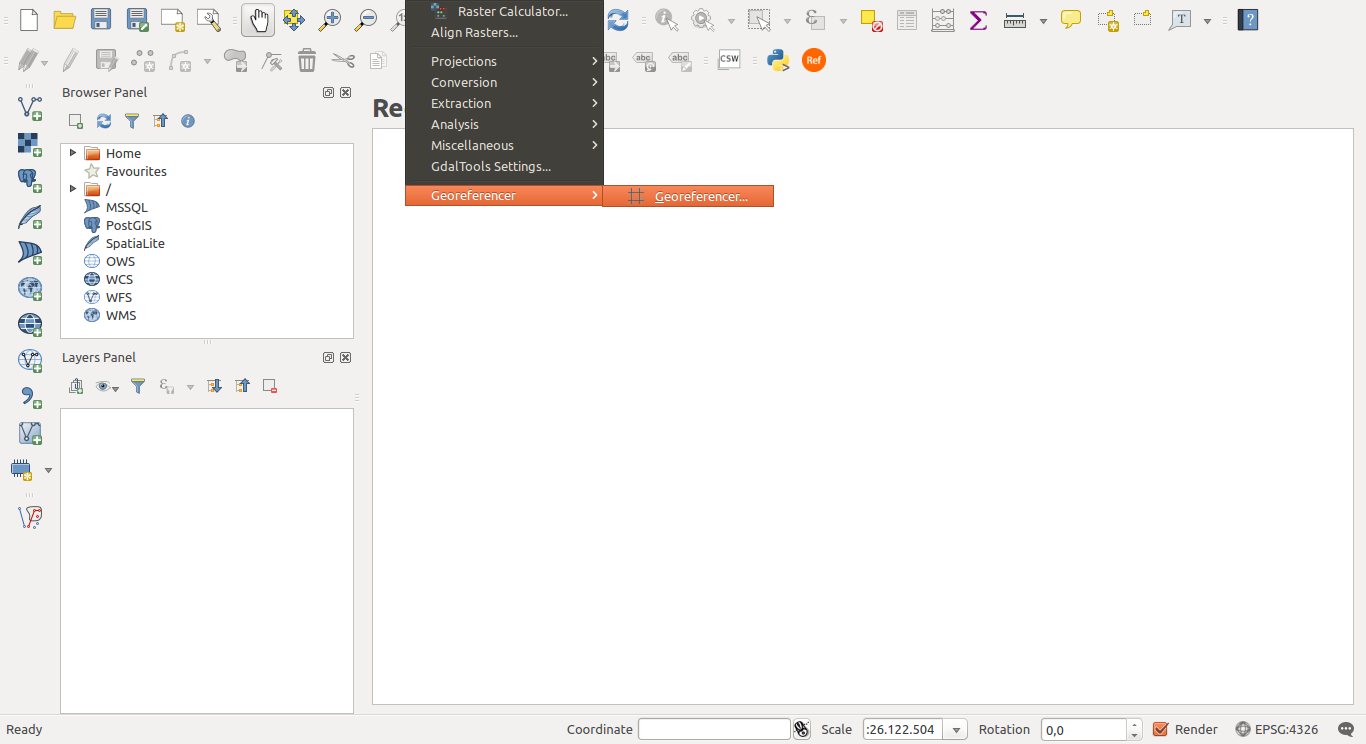
\includegraphics[width=1\textwidth]{./resources/021-georef-menu-exists}
    \caption{Menu \textit{Georeferencer} Muncul}
    \label{fig:georefmenuexists}
  \end{figure}
  
  Setelah memilih menu \verb|georeferencer| maka akan muncul jendela seperti pada gambar \ref{fig:georefwin}.
  
  \begin{figure}[H]
    \centering
    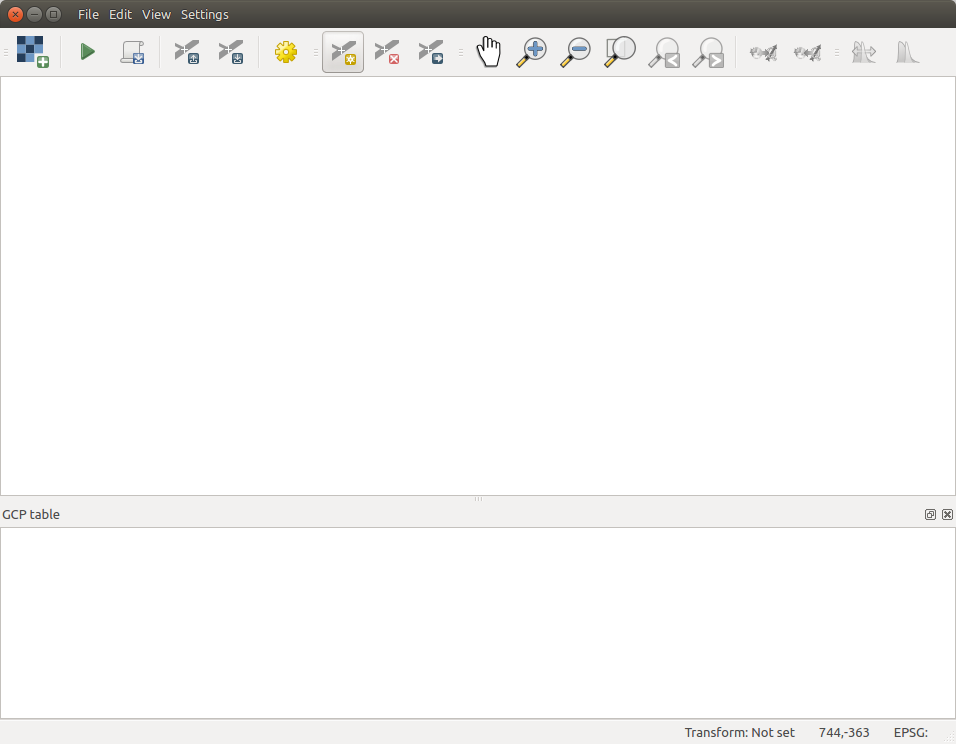
\includegraphics[width=1\textwidth]{./resources/022-georef-win}
    \caption{Jendela \textit{Georeferencer}}
    \label{fig:georefwin}
  \end{figure}
  
  \item Pada jendela \textit{georeferences}, klik \verb|File > Open Raster|. Kemudian pilih peta yang akan di georeferensi. Biasanya dalam bentuk JPG, atau GIF, atau bentuk format gambar yang lain yang didukung. Setelah membuka file \textit{raster} / gambar yang akan di georeferensikan, maka akan muncul gambar yang siap untuk diberikan koordinatnya seperti pada gambar \ref{fig:georeftif}
  
  \begin{figure}[H]
    \centering
    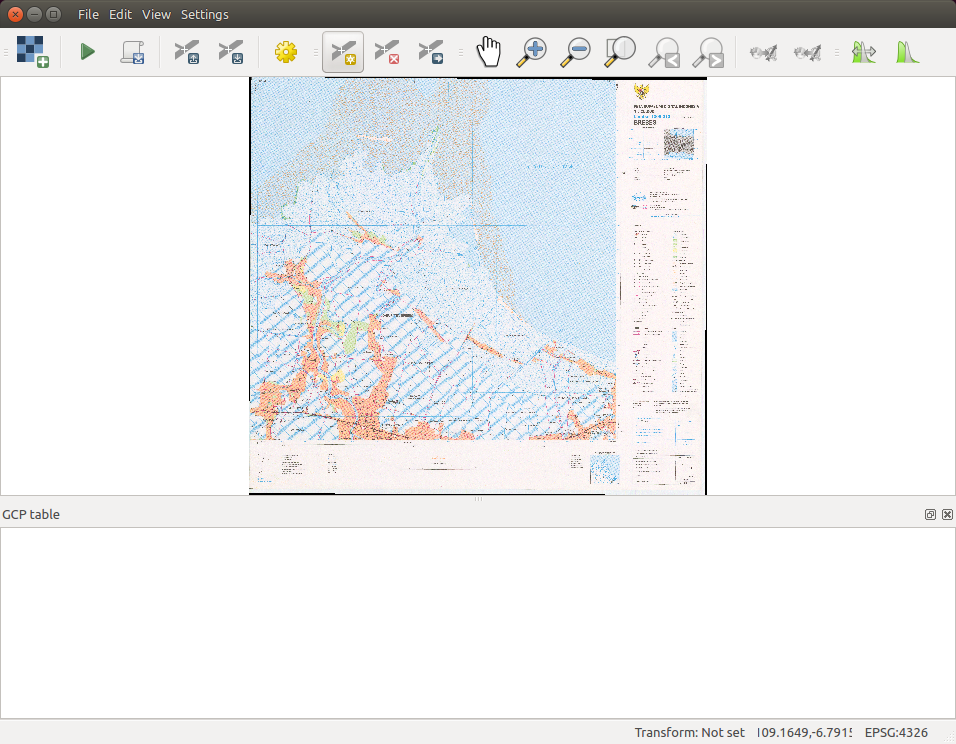
\includegraphics[width=1\textwidth]{./resources/023-georef-tif}
    \caption{\textit{File} TIF Yang Siap Untuk Digeoreferensikan}
    \label{fig:georeftif}
  \end{figure}
  
\end{enumerate}